\chapter{Cadre du stage}

\section{Présentation de l'entreprise d'accueil}
Créée en 2003 par Laurent Py et Bruno LEGEARD, la société LEIROS est spécialisée dans le test logiciel. Elle est issue du projet Smart Testing\texttrademark ~au LIFC\footnote{Laboratoire d'informatique de Franche-Comté}. L'objectif premier de LEIROS a été d'industrialiser le projet Smart Testing\texttrademark.  LEIROS a ensuite changé de nom pour devenir Smartesting en juin 2008. En septembre 2008, Smartesting ouvre sa filiale à Bangalore en Inde. Smartesting compte environ trente-cinq personnes dont onze dans le service R\&D \footnote{Recherche et développement}.

\begin{figure}[!ht]
\centering
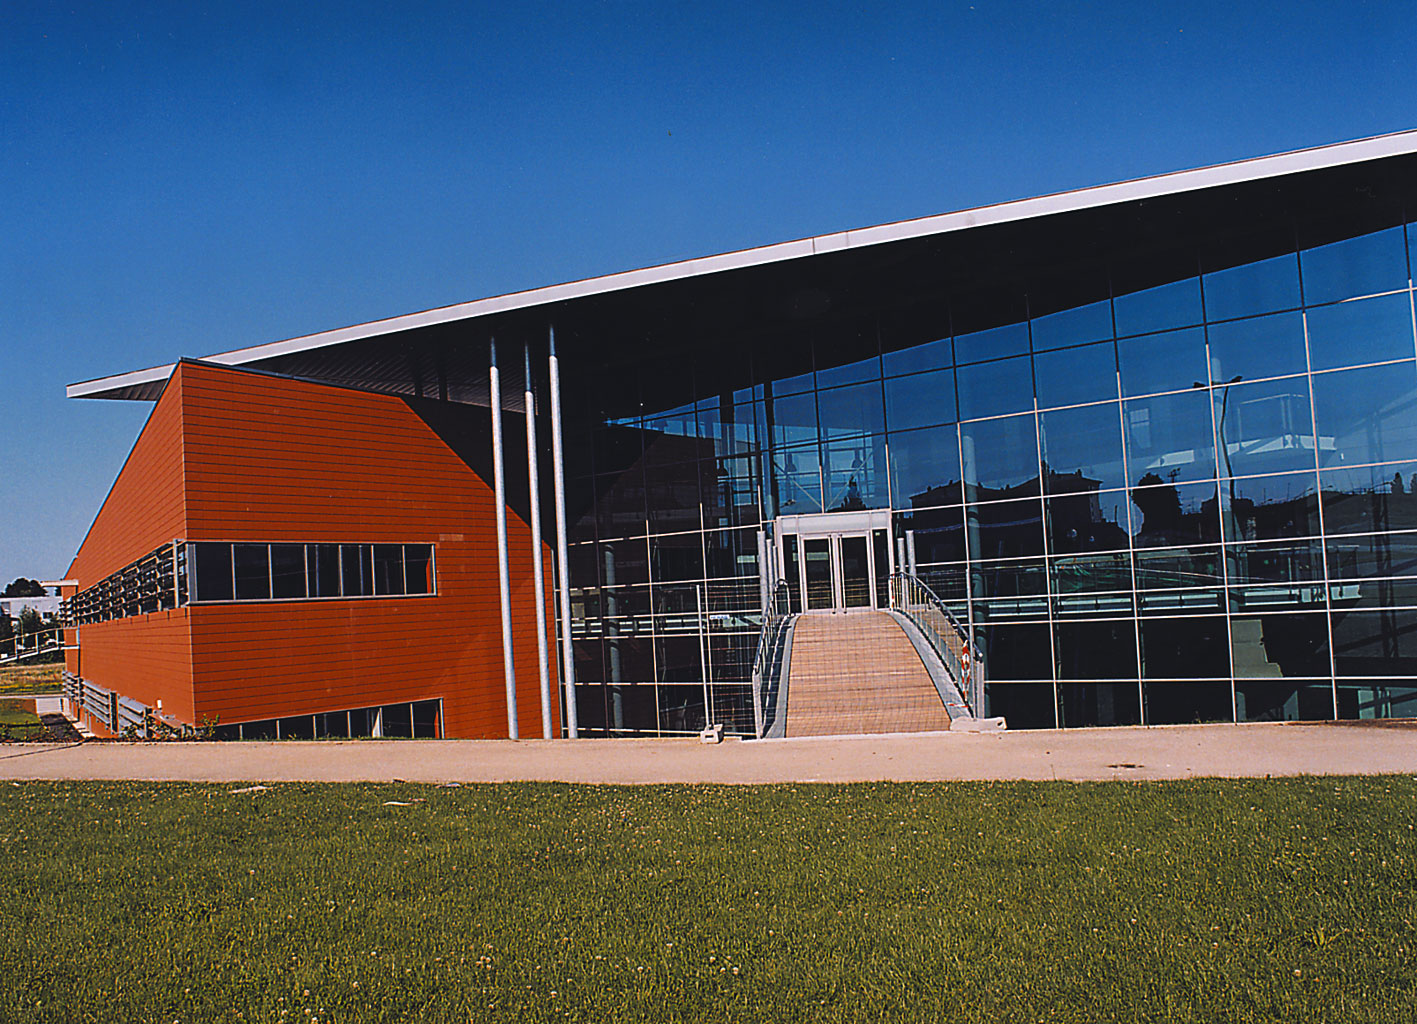
\includegraphics[width=.55\textwidth]{Illustrations/temis.jpg}
\caption{Centre Temis à Besançon}
\label{figure:temis}
\end{figure}

\subparagraph*{}
Smartesting est implantée dans différents points stratégiques. En France, le siège social ainsi que le centre R\&D sont à Besançon dans les locaux de l'hôtel d'entreprises Temis Innovation(cf. figure \ref{figure:temis} p.\pageref{figure:temis}). Ainsi la R\&D reste proche géographiquement de l'université et de la recherche qui y a lieu. À Paris et à Amsterdam aux Pays-Bas se trouvent les agences où travaillent les commerciaux et les avant-vente. Smartesting s'est implantée à Bangalore, en Inde où elle compte réaliser la moitié de son chiffre d'affaires en 2010 grâce au boom de l'offshore où le marché du test logiciel est en pleine expansion.

\subparagraph*{}
Smartesting développe dans le secteur grandissant du test logiciel. Ce marché devrait atteindre 13 milliards de dollars en 2010 (selon une étude de Gartner). Le test logiciel, en particulier le test fonctionnel devient une phase clé du développement logiciel. Des besoins très stricts pour les milieux bancaires par exemple obligent ces entreprises à faire appel à des ingénieurs et des architectes de test afin de concevoir les tests logiciels qui permettront par exemple de garantir la stabilité, la non régression et le bon fonctionnement de gros projets. Smartesting propose Test Designer, une solution de génération automatique de référentiels de test à plusieurs niveaux.

\begin{figure}[!ht]
\centering
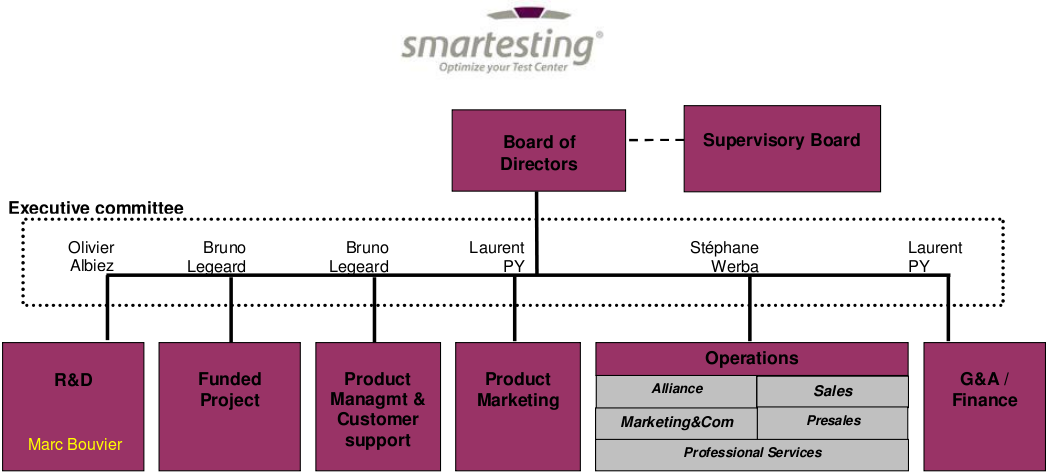
\includegraphics[width=\textwidth]{Illustrations/Organigramme_with_me.png}
\caption{Organigramme de la société Smartesting}
\label{figure:Organigramme de Smartesting}
\end{figure}

\subparagraph*{}
L'entreprise est organisée autour d'un directoire de trois personnes : Laurent PY, Bruno LEGEARD et Stéphane WERBA. Je travaille dans le service de R\&D{}\ de Smartesting.  L'équipe est composée de 11 ingénieurs développeurs qui améliorent sans cesse le produit Test Designer ainsi que les connecteurs et les publishers y sont développés. L'équipe fonctionne autour de méthodes Agiles, en particulier eXtreme Programming. Ces sujets seront développés dans les sections qui vont suivre.

\pagebreak

